\chapter{Desenvolvimento}
\chapter{Metodologia}

Este trabalho se trata de um processo de desenvolvimento pelo do autor de maneira autônoma, dado que os tópicos de programação e alguns detalhes de implementação são por natureza de livre implementação, tornando este trabalho por grande parte um trabalho exploratório. 

\section{A base do projeto}

Para implementação do sistema proposto, é necessário entender que deseja-se que os resultados do sistema, as redes de petri, sejam acessíveis em várias plataformas, visando-se generalização. Entende-se assim que deve-se haver um motor capaz de executar estas redes e seu funcionamento em suas respectivas plataformas. Em computadores de uso geral, e em sistemas embarcados torna-se atrativo uma implementação na forma de uma biblioteca em linguagem C, pois a maioria dos sistemas embarcados funcionam com \textit{toolchains}\footnote{Conjunto de ferramentas que possibilitam a programação e manuseio de programas para uma plataforma e/ou arquitetura de computador específica.} em C, e também pois abre-se as portas para que outros ambientes e linguagens de programação utilizem esta biblioteca. Isto é possível pelo fato de C ser de baixo nível e seguir padrões estabelecidos de arquivos e execução de código no geral, tornando possível que linguagens de mais alto nível possam fazer \textit{bindings}\footnote{Sistema onde se mapeia de forma diretas funções, variáveis e definições de código entre sistemas/ambientes de programação diferentes, possibilitando interoperabilidade entre elas} para com a biblioteca. 

Mais ainda, outro motor importante é a capacidade de executar tais redes em plataformas distintas, onde a portabilidade da biblioteca em C torna-se difícil, como os PLC's comentados anteriormente, onde a lista de instrução é mais comum do que a linguagem C. A lista de instrução, tanto pela difusão quanto pelo baixo nível de abstração, um candidato preferido para alvo de compilação, assim a rede pode ser editada, simulada e testada em um computador de uso geral, por exemplo, e então compilada para lista de instrução, que deve ser gerada de forma a garantir funcionalidade igual a da biblioteca em C.

O baixo nível de abstração da lista de instrução ainda possibilita que esta seja usada como fonte para compilação posterior por ferramentas de terceiros para suas plataformas alvo, abrindo mais funcionalidade para esse tipo de sistema de trabalho. Por exemplo, lista de instrução é comumente compilada para \textit{Ladder} de forma intercambiável, ou seja, é um processo bidirecional, comportamento desejado por desenvolvedores, dado que \textit{Ladder} é uma linguagem visual simples e de mais fácil desenvolvimento do que a lista de instrução pura.

Para implementação da representação das redes, da dinâmica e da compilação será utilizada a linguagem C bem como um sistema de compilação para a biblioteca usando ferramentas básicas no padrão POSIX\nocite{posix}, em especial do projeto GNU \cite{gnu} sendo elas o compilador \textit{gcc}, e para \textit{build}\footnote{Processo organizado de construção de um programa ou biblioteca a partir de diferentes arquivos fonte, que são compilados e ligados conforme a necessidade do projeto.} o \textit{Make}.

% \section{Parte visual}

% No que se refere ao aspecto visual, temos o desenvolvimento de uma aplicação de edição para qual foi tomada inspiração do trabalho anterior Petrilab \cite{de2015petrilab} bem como o editor de texto Visual Studio Code \cite{vscode}. Para o desenvolvimento desta aplicação devemos pensar que a mesma será utilizada em computadores desktop, será escolhido assim um framework visando funcionamento em diversos sistemas operacionais, facilidade e tendencias modernas, como o framework Flutter\cite{flutter}. 

% O mesmo possui uma metodologia moderna de desenvolvimento de aplicações visuais bem como a capacidade de ter como linguagem de programação o Dart, qual possui interoperabilidade com C, podendo assim a aplicação visual utilizar a biblioteca em C para simulação a rede de petri criada.

\section{Rede de petri}

Quanto a definição do tipo de rede de petri adotada neste trabalho, serão adotadas redes de petri com extensões específicas e utilidade geral de e industrial, garantindo maior flexibilidade no design. A definição destas extensões e os detalhes de implementação serão discutidos e embasados conforme trabalhos anteriores bem como a experiência prática do autor.

\section{Compilador de lista de instrução}

Lista de instrução é um tipo de programação relativamente difundida e portanto bem generalizada, mas ainda assim há diferenças entre fabricantes. Em vista disto, a implementação do compilador de rede de petri para lista de instrução proposta neste trabalho irá utilizar uma implementação específica, sendo esta a referência da fabricante WEG para o PLC TPW04 \cite{wegtpw04}, sendo este um modelo amplamente utilizado em meio industrial e também de fácil acesso em educacional e acadêmico. Futuros trabalhos podem partir da mesma referência para implementação de compiladores para mais arquiteturas de PLC's, dada que as diferenças de implementação são pequenas entre tipos de plataformas e fabricantes diferentes devido a norma IEC 61161-3 \cite{IEC611313}.  

\section{Publicação}

Todo o trabalho desenvolvido nesta obra será versionado e disponibilizado no repositório "pnet" \cite{github-pnet} via Github \cite{github}, sob a licença domínio público MIT \cite{mit-license}.

% Todo o trabalho desenvolvido nesta obra será versionado e disponibilizado como repositórios distintos via Github \cite{github}, todos sob a licença domínio público MIT \cite{mit-license}, sendo estes repositórios o da biblioteca C \cite{github-pnet}, da aplicação visual Flutter \cite{github-petricad} e do plugin Flutter que irá encapsular a funcionalidade da biblioteca em C via bindings utilizando as capacidades da linguagem Dart \cite{github-pnet-dart}.

% Começando pela base, é desenvolvido primeiramente a biblioteca em C, onde serão definidos a estrutura, checagem, serialização e armazenamento e dinâmica/simulação da rede, que irão compor a biblioteca e permitir que ela seja de uso genérico conforme a especificação. 

% Ao fim será desenvolvido o algoritmo que se utilizará da estrutura de dados da rede petri para realizar a compilação para lista de instrução, referência WEG TPW04 \cite{wegtpw04}.

\section{Biblioteca C}

No desenvolvimento da biblioteca em C, como qualquer outro tipo de programa, uma das primeiras coisa a serem feitas é a definição de uma estrutura de dados, como discutido previamente, iremos implementar a rede de petri em código utilizando a representação matricial. Implementada a funcionalidade das matrizes podemos definir a estrutura da nossa rede de petri e por fim, definir os algoritmos que irão realizar a funcionalidade desejada da biblioteca.

Como padrão serão definidas para cada estruturas de dados um \lstinline{struct} que será inicializado a partir de uma função de criação de forma dinâmica, retornando um ponteiro para a estrutura.

\subsection{Representação matricial}

Primeiramente define-se a estrutura primitiva da matriz, a qual irá comportar o tamanho e \textit{array} dinâmico de memória de duas dimensões. Escolhe se \lstinline{size_t} pois este comporta o maior valor de tamanho disponível na arquitetura a ser compilada para e \lstinline{int} para os valores da matriz, visto que todas as matrizes que irã comportar a representação matricial podem ter valores positivos e negativos.

\lstinputlisting[
    language=C,
    caption={Estrutura C da matriz},
    sourcePrefix={Fonte: },
    source={Do autor.},
    label={code:matrix}
]{code/matrix.c}

Com a definição da matriz, pode-se pensar nas definições dos arcos, para isso em uma matriz $A$, $n$ por $m$, com $n$ sendo a quantidade de linhas e lugares, e $m$ sendo a quantidade de colunas e transições, arcos de tipo peso podem ser dados como no seguinte exemplo.

$$ A = 
\begin{bmatrix}
	-1 & 0\\
	 1 & -1\\
	 0 & 2
\end{bmatrix}
$$

Onde pode-se ver três lugares e duas transições, onde a primeira transição retira uma ficha do primeiro lugar e a coloca no segundo lugar, e a segunda transição retira do segundo lugar e coloca duas fichas no terceiro lugar.

Uma das problemáticas que irá surgir é a que a rede de petri permite dois arcos de peso de um mesmo lugar para uma mesma transição, e nossa representação não a comporta, pois para retirar e colocar uma ficha, devemos marcar como zero, mas zero significa nenhum arco, para tanto, divide-se a matriz em duas, uma matriz $A_p$ para arcos de peso positivo, que colocam fichas em lugares e outra matriz $A_n$ para arcos negativos, que retiram fichas de lugares. Assim teremos para o mesmo exemplo: 

$$ A_p =
\begin{bmatrix}
	-1 & 0\\
	 0 & -1\\
	 0 & 0
\end{bmatrix}
$$

$$ A_n =
\begin{bmatrix}
	 0 & 0\\
	 1 & 0\\
	 0 & 2
\end{bmatrix}
$$

Assim temos a distinção entre arcos não existentes e dois arcos distintos entre um lugar e uma transição. 

Para os arcos negados e de \textit{reset} a representação é mais simples, pois devemos apenas marcar com um, para um arco, ou zero, para sem arco. Exemplo de um arco negado da primeira transição para com o terceiro lugar.

$$ A_i =
\begin{bmatrix}
	 0 & 0\\
	 0 & 0\\
	 1 & 0
\end{bmatrix}
$$

E um exemplo de um arco \textit{reset} que após o disparo da primeira transição zera todos os lugares.

$$ A_r =
\begin{bmatrix}
	 1 & 0\\
	 1 & 0\\
	 1 & 0
\end{bmatrix}
$$

Tendo já os arcos, podemos agora definir o estado inicial da rede de petri, que são as fichas iniciais que alguns lugares possuem conforme o design do autor da rede. É relativamente simples, apenas uma matriz unidimensional com os valores para cada lugar. Exemplo de lugar inicial de um de três lugares.

$$
P_i = 
\begin{bmatrix}
	 1 & 0 & 0
\end{bmatrix}
$$

Também para as transições é necessário definir o valor da temporização dos arcos, que também é uma matriz unidimensional. Exemplo de um tempo de \SI{5}{s} para a primeira de duas transições.

$$
T = 
\begin{bmatrix}
	 5000 & 0
\end{bmatrix}
$$

Para as entradas da rede define-se, como nos arcos, uma matriz de relação entre entradas e transições. Assim define-se uma matriz de $n$ linhas, as entradas, por $m$ colunas, as transições, e também deve se definir uma forma de codificar em um número inteiro, devido à implementação da matriz, o tipo de evento a ser usado, para isso define-se um enumerador C com as três possíveis bordas propostas, de subida, descida e ambas.

\lstinputlisting[
	language=C,
	caption={Codificação dos eventos de entrada},
	sourcePrefix={Fonte: },
	source={Do autor.},
	label=code:event
]{code/event.c}

Observa-se que definimos também um evento nulo, zero, que simboliza nenhuma relação, e um evento \lstinline{max}, que tem como função apenas a checagem, que será vista mais a frente. Note também como a borda de ambos, \lstinline{any_edge}, é a soma do valor das outras duas bordas, assim que utilizar a biblioteca para criação de redes de petri pode utilizar do operador lógico ``ou'' para indicar verbosamente ambas as bordas, \lstinline{pnet_event_any_edge = pnet_event_pos_edge | pnet_event_neg_edge}.

Um exemplo de matriz onde deseja-se que a transição um seja acionada somente quando haja uma borda de subida da entrada dois.

$$
I_{in} = 
\begin{bmatrix}
	0 & 0\\
	1 & 0
\end{bmatrix}
$$

As saídas são definidas como a quantidade de fichas maior ou igual necessárias a ativação, portanto nenhuma codificação é necessária, apenas o valor numérico, assim tempos uma matriz de $n$ linhas, lugares, or $m$ colunas, saídas. Um exemplo caso desejarmos que a saída um seja acionada quando o número de fichas no lugar três seja maior ou igual a quatro.

$$
O_{out} = 
\begin{bmatrix}
	0 & 0\\
	0 & 0\\
	4 & 0
\end{bmatrix}
$$

Com estas definições podemos então definir a nossa estrutura em C da rede de petri, listagem de código \ref{code:pnet}.

\lstinputlisting[
	language=C,
	caption={Estrutura C da rede de petri},
	sourcePrefix={Fonte: },
	source={Do autor.},
	label=code:pnet
]{code/pnet.c}

Nota-se a presença de mapas, estes são as matrizes até então mencionadas, mesmo as fichas inicias e temporização, o restante dos valores são pertinentes ao processamento e execução de rede e serão explorados posteriormente. 

\subsection{Checagem}

Dada a estrutura da rede de petri a primeira coisa a ser pensada é que as matrizes são de livre preenchimento e portanto podem haver definições de redes de petri inválidas, comportamento que deve ser devidamente checado para que a rede de petri possa ser minimamente executável, para tanto implementa-se um algoritmo de checagem baseado nas definições propostas, na capacidade de execução e viabilidade do ponto de vista de \textit{software}.

Destaca-se um problema em particular, que seria a mínima rede válida permitida, pois diz respeito as capacidades permitidas para execução da rede sem erros e garantindo a comportamento desejado dadas as especificações. Para isto vamos considerar quais seriam as matrizes opcionais da rede de petri. Entradas e saídas são opcionais por não interferem no funcionamento da rede. Temporização também não é requerida para todas as transições. 

A quantidade de lugares e transições é dada pelos tamanhos das matrizes de arcos e da marcação inicial das fichas, assim ao menos uma dessas deve ser não nula, e mesmo que não hajam arcos, uma rede pode ainda ser válida, com somente lugares e transições, somente um lugar e uma transição ou ainda um único lugar ou única transição. Para uma rede de petri com uma única transição devemos ter ao menos uma das quatro matrizes de arcos, e dado que estas também definem a existência de lugares, pois não podem haver zero linhas em uma matriz, então uma rede de apenas uma transição não é possível neste tipo de implementação, sendo assim a menor rede viável é a de apenas um lugar, a qual pode ser definida apenas pela matriz de marcação inicial.

É interessante ainda expandir essa definição se escolhermos que nossa rede de petri seja passível de execução, sendo necessário assim uma transição e um tipo de arco capaz de alterar a quantidade de fichas, arcos de peso ou arcos de \textit{reset}. Assim então definimos a rede mínima para esta implementação uma rede com no mínimo a matriz de marcação inicial e ao menos umas das duas matrizes de arco, de \textit{reset} ou de peso, as quais podem ser matrizes de minimamente de um por um, sendo assim as redes mínimas as redes de um lugar e uma transição com um arco de peso ou arco de \textit{reset}. 

% imagem

Dadas as especificações e a análise da rede mínima viável, os seguintes pontos devem ser reforçados para criação das redes:

\begin{itemize}
	\item Consistência na quantidade de lugares e transições nas matrizes. Erro se qualquer matriz não for adequada.
	\item Existência de somente números positivos na matriz de arcos positivos. Outros valores serão zerados.
	\item Existência de somente números negativos na matriz de arcos negativos. Outros valores serão zerados.
	\item Existência de somente um ou zero na matriz de arcos negados e arcos de \textit{reset}. Outros valores serão considerados como um.
	\item Existência da matriz de marcações iniciais. Erro se não detectado.
	\item Números negativos de fichas na inicialização dos lugares, interpretado como erro.
	\item Existência de pelo menos um arco de pelo menos um tipo um de arco, garantindo dinâmica na rede. Erro se não detectado.
	\item Números negativos na temporizações das transições, interpretado como erro.
	\item Existência de apenas eventos válidos de entrada. Corrigido para evento nulo, zero, caso contrário.
	\item Existência de apenas um evento de entrada por uma transição. Erro caso contrário.
\end{itemize}

Ao final da checagem, uma variável binária é marcada como um dentro da estrutura da rede de petri, indicando que esta pode-se executada normalmente.  

É importante ressaltar que a criação da rede e sua checagem é referente a esta implementação em específico dada as necessidades de \textit{software}, tipo de rede proposto e limitações, não necessariamente refletindo os conceitos formais de rede de petri mínima e implicações relacionadas.

Também referente a implementação são realizados os seguintes testes práticos na implementação da rede de petri para garantir funcionalidade não só de execução mínima mas também das outras capacidades que irão serão posteriormente desenvolvidas nas seções seguintes.

\begin{itemize}
	\item Teste para retorno não nulo e código de erro ok
	\item Teste para criação com todos os argumentos
	\item Teste para todos os argumentos nulos
	\item Teste para apenas lugares, sem arcos
	\item Teste para autocorreção de valores
	\item Teste para arcos sem peso ou negados
	\item Teste para múltiplas entradas em uma única transição
	\item Teste de sensibilização
	\item Teste de disparo sem arcos de peso ou \textit{reset}
	\item Teste de disparo com entradas para matriz de entrada nulo
	\item Teste de disparo com entradas nulas para matriz de entrada não nula
	\item Teste de disparo de uma única transição com evento de entrada do tipo \lstinline{none}
	\item Teste de falha no disparo
	\item Teste de transição com arco de peso, negados e \textit{reset} e eventos de entrada
	\item Teste de arco de peso e \textit{reset}
	\item Teste para sensibilização de transições sem matriz de entradas e entrada nula para \lstinline{pnet_fire}
	\item Teste de disparo manual
	\item Teste para estado de saída no início
	\item Teste para múltiplas transições mútuas e um arco bidirecional
	\item Teste para estado de saída no final
	\item Teste de rede temporizada sem passar função de \textit{callback}
	\item Teste de acurácia de transições temporizada
	\item Teste de petri multi temporizadas
	\item Testes com redes de petri de demonstração
	\item Testes de serialização de matriz
	\item Testes de desserialização da matriz
	\item Comparação se matriz é igual a desserialização da serialização da matriz
	\item Teste para criação de matrizes grandes
	\item Teste matriz de um por um é igual a desserialização da serialização
	\item Teste de tamanho máximo factível da desserialização da serialização
	\item Teste de desserialização da serialização da rede de petri
	\item Teste de compilação de rede de petri para lista de instrução
\end{itemize}

\subsection{Sensibilização}

Dado uma rede petri válida, para que antes de a executarmos em tempo real, precisamos executá-la uma única vez, um disparo, e para isso necessitamos antes verificar quais transições estão sensibilizadas dado o estado atual, dado pela matriz \lstinline{places}, visto no código \ref{code:pnet}. Para isso utilizaremos um simples algoritmo que irá varrer e comparar os mapas dos arcos de condição, que são os arcos de peso negativos e arcos negados, com o estado atual da rede.

\lstinputlisting[
	language=C,
	caption={Sensibilização das transições},
	sourcePrefix={Fonte: },
	source={Do autor.},
	label=code:sense
]{code/sense.c}

Na implementação primeiramente dizemos que, para determinada transição, ela se encontra sensibilizada por padrão, então verificamos se existem as matrizes dos arcos de condição e para cada tipo de arco, se existe relação entre o lugar e transição atual, e ainda, se o lugar possui a condição necessária, seja de fichas necessárias para os arcos de peso negativo ou zero fichas para o arco negado. Chegando ao final de todas as das condições, se algo não for verdadeiro, a transição será marcada como não sensibilizada.

Note que a matriz das transições \lstinline{sensitive_trasitions} é interna a rede de petri e que a cada verificação de sensibilidade retorna várias transições sensibilizadas, que está em contradição com nossa especificação da seção \ref{section:limitations}, porém será tratada posteriormente na realização de disparos.   

O ponto de entrada para realização análise de sensibilização será uma função distinta denominada \lstinline{pnet_sense}.

\subsection{Disparo}

Dada uma matriz com as transições a serem sensibilizadas é necessário ainda verificar se as transições possuem relação de entrada, caso no qual deverá ser feita uma verificação das bordas de entrada. A verificação das bordas de entrada é feita comparando se o valor atual é diferente do anterior, para isso é necessário guardar o estado anterior das entradas, seria a matriz \lstinline{inputs_last} dada no código \ref{code:pnet}.

O ponto de entrada para realização dos disparos será uma função distinta denominada \lstinline{pnet_fire}, a qual dentro si realiza uma chamada a função \lstinline{pnet_sense}, incorporando assim a lógica completa de disparos, exceto pelos disparos temporizados, que irão ocorrer de forma assíncrona, discutidos na próxima seção. Na função \lstinline{pnet_fire}, também é repassado o valor atual das entradas externas, assim pode-se verificar se houve mudança e portanto, se houver um evento ou uma borda, e se o evento irá contribuir para o disparo de alguma transição. Para isso verifica-se a entrada com o estado anterior e armazena se o resultado na matriz temporária \lstinline{edges}. 

\lstinputlisting[
	language=C,
	caption={Processamento dos eventos de borda de entrada},
	sourcePrefix={Fonte: },
	source={Do autor.},
	label=code:input
]{code/input.c}

Primeiramente para cada transição, se assume que ela está sensibilizada, então se verifica para cada uma se existe um mapa de entrada, caso não ela permanece sensibilizada, caso não, verifica-se se a mesma possui um evento nulo atrelado, caso qual pulamos e a transição continua sensibilizada, caso contrário, se a borda for a mesma especificada pela matriz de entrada então a mesma continua sensibilizada. Caso nenhuma dessas condições não for verdadeira, a transição é marcada como dessensibilizada.   

\lstinputlisting[
	language=C,
	caption={Sensibilização de transições pelos evetnos de entrada},
	sourcePrefix={Fonte: },
	source={Do autor.},
	label=code:inputtran
]{code/input_tran.c}

É interessante notar como no código \ref{code:event}, as bordas de subida e descida são distintas, mas a borda ambos é a soma do valor delas, basta realizar a operação lógica ``e'' para poder determinar o resultado, se o valor da matriz de entrada for igual ao detectado, então ``e'' será verdadeiro, e se o valor da matriz for para ambos, se a detectada for, por exemplo, de subida, então teremos \lstinline{0x03 & 0x01}, que será também verdadeiro, como pode ser visto na linha 21 do código \ref{code:inputtran}.

Tendo agora duas matrizes, a matriz de transições sensibilizadas pelos arcos condicionais e a matriz de transições sensibilizadas pelas entradas, portanto as transições que devem ser disparadas serão o resultado lógico ``e'' de ambas as matrizes.

\lstinputlisting[
	language=C,
	caption={Disparo das transições},
	sourcePrefix={Fonte: },
	source={Do autor.},
	label=code:fire
]{code/fire.c}

No código \ref{code:fire} linha 2 vemos a operação lógica ``e'', e temos então a matriz de transições para executar, porém, conforme mencionado na seção \ref{section:limitations}, destas, podemos executar ao máximo uma transição, então a partir do momento que temos uma transição não temporizada que está apta, esta será executada e o irá quebrar o laço de repetição, assim outras transições não serão executadas. Aqui vê se a ambiguidade de que a primeira transição que for declara tem prioridade, devido ao laço de repetição, essa é a justificativa para implementação de prioridade de transições, que vem do tipo de rede de petri priorizada, porém, novamente, a escolha deste tipo de implementação é justificada pela finalidade de aplicação, assumindo que esse tipo de ambiguidade não será de grande problema. 

A função \lstinline{pnet_move} realiza a movimentação das fichas conforme os arcos atuadores, os arcos de peso negativo e positivo e o arco \textit{reset}, a forma como a movimentação é alcançada pode ser dada em termos matemáticos, para os arcos de peso, de uma única matriz $A$ com arcos positivos e negativos, e uma matriz $T$ que representa a transição a ser disparada, o resultado da movimentação das fichas pode ser dado como: 

$$
T_{t=0} = \begin{bmatrix}
	1 & 0 & \dots
\end{bmatrix}
$$

$$
P_n = P + T \cdot A^T
$$

Onde $a$ é uma célula, $m$ o índice da coluna, $A^T$ a transposta de, $P$ a matriz dos lugares atuais e $P_n$ os novos lugares após o disparo.

Esse algoritmo funciona de forma adequada, exceto pelo fato da multiplicação matricial ser extremamente custosa para grandes matrizes. Como se sabe o tipo de matriz que temos, podemos começar extraindo a coluna da matriz de arcos que representa a única transição a ser disparada, diminuindo drasticamente o cálculo envolvido. Com essa nova matriz unidimensional, pode-se simplesmente realizar a soma diretamente aos lugares da rede de petri. 

Para a implementação desse trabalho necessitamos primeiramente extrair as colunas da matriz de arcos positiva e negativa e então realizar a soma.

$$
a = A(m=t)
$$

Onde $A_n$ são os arcos negativos e $(m=t)$ representa a coluna da transição $t$, sendo $a_n$ um vetor de $m$ elementos e uma única linha.

$$
P_n = \left(P + a_n^T + a_p^T\right) \odot \neg a_r
$$

Onde $a_n$ são a coluna transição dos arcos negativos, $p$ positivos e $r$ de \textit{reset}, $\odot$ é a multiplicação de elemento a elemento, diferente da multiplicação matricial normal, e $\neg$ a negação lógica dos elementos matriciais. Em código temos:

\lstinputlisting[
	language=C,
	caption={Movimentação das fichas},
	sourcePrefix={Fonte: },
	source={Do autor.},
	label=code:move
]{code/move.c}

\subsection{Temporização e assincronia}

Nota-se que no código \ref{code:fire} que a transição só é de fato disparada caso não haja matriz de temporização ou quando a temporização para a mesma for zero, porém quando há temporização, a mesma deve iniciar o processo de contagem juntamente com outras transições que possam começar a contar, isso pelo fato de que o início da contagem pode ocorrer de forma simultânea, somente o disparo das transições deve ser único, comportamento que pode-se tornar complexo, para tanto deve se visionar um sistema de contagem que garanta o mesmo.

Dentro deste \textit{thread} código erá executado para efetuar a contagem das transições temporizadas quando forem sensibilizadas, porém, como visto, isso pode levar a situações onde podem haver múltiplas transições simultâneas. Para lidar com esse aspecto e facilitar a organização e contagem destas transições, é implementado uma estrutura de dados específica, uma fila priorizada. 

A implementação da fila é feita da seguinte forma, uma lista ligada que guarda elementos especiais, responsáveis pela metainformação de cada transição temporizada, e que trabalha a inserção e retirada dos elementos conforme a prioridade da contagem atual, de forma que os elementos com menor quantidade de tempo restante fiquem ao fim da lista, pois tem maior prioridade, assim podemos apenas verificar o último elemento da lista para saber se o mesmo deve ser disparado ou não, sem necessidade de checar o restante dos elementos.

Os elementos da lista ligada são transições, que são da seguinte forma:

\lstinputlisting[
	language=C,
	caption={Elemento de transição temporizado},
	sourcePrefix={Fonte: },
	source={Do autor.},
	label=code:transition
]{code/transition.c}

Onde guarda-se o número da transição, o tempo inicial $t_0$ onde a transição foi ativada e o tempo total de temporização $t$. Para realizar a inserção na lista teremos uma função \lstinline{transition_queue_push}, qual insere os elementos de menor $t_0 + t$.

\lstinputlisting[
	language=C,
	caption={Inserção de elemento na lista priorizada por tempo},
	sourcePrefix={Fonte: },
	source={Do autor.},
	label=code:transition
]{code/transition.c}

Percorre-se a lista com um laço de repetição, começando ao final, onde estão as transições mais próximas de executar, em direção ao início. Verifica-se então se a transição já está presente na lista, se sim retornar da chamada, pois não há necessidade de inserção. Se o tempo final $t_0 + t$ for menor que o da transição atual, inserir o elemento a frente daquela transição, e caso se chegar ao início da lista sem que não seja inserido nada, inserir ao início da lista como a transição mais longe de ser executada. Tal processo é assegurado pelo uso de um \lstinline{mutex} definido para a instância da lista, evitando possíveis erros por \textit{race conditions}.

Essa chamada foi usada no código \ref{code:fire} linha 21, onde verifica-se que a inserção é realizada para quantas transições forem sensibilizadas naquele momento.

Para retirada da transição da lista implementa-se a chamada \lstinline{transition_queue_pop}, que é definida como:

\lstinputlisting[
	language=C,
	caption={Retirada de elemento na lista priorizada por tempo},
	sourcePrefix={Fonte: },
	source={Do autor.},
	label=code:pop
]{code/pop.c}

Na linha 1 obtém se o tempo atual em milissegundos usando a função \lstinline{clock}, que nos dá a quantidade de tempo passado desde o início do programa até o momento atual. Então verifica-se se o último elemento da lista é passível de ser retirado, então compara-se o tempo passado até o momento desde a inserção da transição com o tempo de temporização total. Caso tenha sido alcançado, a função retorna sucesso e o elemento pode ser acessado pelo ponteiro de referência passado como parâmetro, caso contrário, o retorno é zero.

Assim, a contagem no \textit{thread}, dado pela própria estrutura da rede de petri, pode ser feita com a seguinte rotina de execução:

\lstinputlisting[
	language=C,
	caption={Rotina de execução do \textit{thread} temporizador},
	sourcePrefix={Fonte: },
	source={Do autor.},
	label=code:thread
]{code/thread.c}

Observa-se que a rotina é executa de forma infinita, sempre tentando retirar elementos da fila priorizada, caso não consiga, o laço simplesmente se repete. Lembrando que este processo ocorre de forma paralela ao código da rede. Caso o retorno seja verdadeiro podemos verificar se a transição ainda encontra se sensibilizada, comportamento desejado, pois se ela deixar de ser sensibilizada então a mesma não deve ser disparada. Caso se encontrar, então disparamos a rede e executamos o \textit{callback} de retorno, deixando o usuário da rede atento que uma transição foi executada de forma assíncrona, fora to tempo de execução da chamada \lstinline{pnet_fire}. 

Tal \textit{callback} é definido na criação da rede, visto no código \ref{code:pnet} juntamente a fila priorizada, uma simples função que é executada de forma assíncrona e recebe como parâmetros os dados do usuário, dados no momento da criação, e o número da transição que foi executada, que pode ser utilizado para lógicas auxiliares de escolha do usuário.

As funções de checagem de sensibilização e de movimentação de fichas são \textit{thread} safe também, graças a um outro \textit{mutex} localizado também na estrutura rede de petri, assim, quando as transições temporizadas ocorrerem, elas não entrarão em conflito com as transições instantâneas da execução normal. 

Com essa última definição chegamos ao final da estrutura dada no código \ref{code:pnet}, onde cada elemento definido além das matrizes de definição, os mapas, é necessário para que a rede funcione como um todo.

\subsection{Serialização de matrizes}

A serialização de dados é bastante simples quando têm-se acesso ao baixo nível, como é o caso da linguagem C, onde podemos ler dados da memória e interpretá-los de maneira livre. Uma das formas de fazer isso é utilizando uma técnica chamada \textit{pointer casting}, onde uma estrutura é definida e então atrelada como ponteiro a uma região de memória, funcionando para leitura e escrita, isso se torna uma forma conveniente de se serializar e desserializar dados. 

As matrizes que compõe nossa rede de petri ocupam um espaço relevante de memória, portanto guardar uma matriz $n$ por $m$ de números inteiros ocuparia minimamente $n\cdot m \cdot 4$ \textit{bytes}, tamanho que cresce exponencialmente, porém, como a maioria das matrizes possui muitos valores nulos, devido às relações de arcos e marcação inicial, podemos tomar vantagem disso e gravar apenas os valores não nulos, usando marcadores de linha e coluna.

Define-se assim então para cada matriz um cabeçalho de memória, onde serão contidas a quantidade de linhas e colunas e então os valores não nulos.

\lstinputlisting[
	language=C,
	caption={Cabeçalho da serialização de matriz},
	sourcePrefix={Fonte: },
	source={Do autor.},
	label=code:mfile
]{code/matrix_file.c}

Como estamos usando matrizes de número inteiro, será fixado o tamanho em \textit{bits} das variáveis como \lstinline{uint32_t} para índices e \lstinline{int32_t} para os valores.

Os valores serão escritos da seguinte forma, marca-se primeiro a linha, caso haja no mínimo um valor não nulo nela, usando o índice da linha e marcando o último \textit{bit} da representação binária do número, como forma de diferenciar que este número se trata do índice da linha. Assim o número a ser gravado será de \lstinline{n = c | 0x80000000}, e a leitura pode ser feita como \lstinline{c = n & ~0x80000000}. 

Dada a linha, cada valor da linha será um par de dois números, o índice da coluna e o valor.

Para seguinte matriz de exemplo teremos:

$$
\begin{bmatrix}
	0 & 0 & 0 & 1\\
	64 & 0 & 0 & 1\\
	0 & 0 & 0 & 0\\
	0 & 0 & $0x7FFFFFFF$ & 16
\end{bmatrix}
$$

$$
Ser =
\begin{Bmatrix}
	4, 4, $0x80000000$, 3, 1, $0x80000001$, 0, 64, 3, 1, $0x80000003$, 2, $0x7FFFFFFF$, 3, 16
\end{Bmatrix}
$$

Assim, dado um \textit{array} de memória de tipo \lstinline{uint32_t *} de tamanho \lstinline{size_t bytes}, podemos realizar um casting conforme o código \ref{code:mfile} para encontrar o tamanho da matriz e assim pré alocar a matriz para ler novamente os dados. 

\subsection{Serialização da Rede de petri}

Dada a serialização das matrizes, a rede de petri torna-se fácil, pois é composta de várias matrizes, deixando somente a definição de alguns metadados necessários. O cabeçalho do arquivo pode ser dado como:

\lstinputlisting[
	language=C,
	caption={Cabeçalho de arquivo da rede de petri},
	sourcePrefix={Fonte: },
	source={Do autor.},
	label=code:header
]{code/header.c}

Nota-se que o primeiro membro, \textit{magic}, trata-se de uma identificação visual, este guarda quatro caracteres de texto de valor sempre ``PNET'', de forma a indicar que este arquivo é um arquivo de tipo rede de petri, seguido do número de versão do arquivo, que têm-seu caso de uso caso a partir deste valor no cabeçalho ocorra mudanças no futuro, os programas podem alterar a leitura e escrita com base no número de versão, dando flexibilidade e opções de versionamento. 

Temos o valor binário de validez da rede de petri, seguido do valor de tamanho das matrizes, que como discutido anteriormente foi dado como de trinta e dois \textit{bits}, \lstinline{0x20}, mas poderia ser dado como matrizes de dezesseis \textit{bits}, \lstinline{0x10}, ou outros tamanhos caso a necessidade de armazenamento de memória.

O campo \lstinline{size} armazena o valor total de \textit{bytes} ocupado pela serialização rede excepto pelo cabeçalho fixo, ou seja, a partir do campo \lstinline{neg_arcs_map_size}. Existe também a checagem CRC32 \cite{crc32} dos dados serializados, exceto pelo cabeçalho, para que se possa detectar erros por corrupção de memória. E finalmente as quantidades de elementos, transições, lugares, entradas e saídas, e então as matrizes e seus tamanhos em \textit{bytes}, que compõem nossa rede de petri.

Matrizes serializadas
\begin{itemize} 
	\item Matriz de arcos de peso negativos
	\item Matriz de arcos de peso positivos
	\item Matriz de arcos negados
	\item Matriz de arcos de \textit{reset}
	\item Matriz de marcação inicial
	\item Matriz de temporização das transições
	\item Matriz de entrada
	\item Matriz de saída
	\item Matriz de estado atual dos lugares
	\item Matriz de transições sensíveis
	\item Matriz de estados das saídas
	\item Matriz do estado anterior das entradas
\end{itemize}

Como temos um número fixo de matrizes, basta realizar a leitura do tamanho de cada uma, e então a leitura da matriz em si. 

Para este arquivo, dado o nome da biblioteca e do indicador no cabeçalho, sua extensão será denominada \lstinline{.pnet}. Um arquivo preenchido tem o seguinte formato visto sobre um analisador hexadecimal:

\begin{figure}[h!]
	\centering
	\caption{Visão do arquivo pnet em um analisador hexadecimal}
	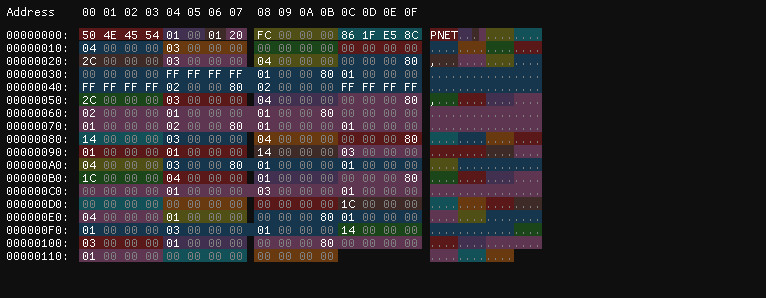
\includegraphics[width=16cm]{images/hexfile.png}
	\label{fig:hexfile}
\end{figure}

\pagebreak

\section{Algoritmo de compilação para lista de instrução}

A compilação para lista de instrução foi baseada no método de compilação para \textit{Ladder} apresentado no trabalho Petrilab \cite{de2015petrilab}, porém qui, para lista de instrução. Fato que é possível devido à característica de que programação \textit{Ladder} pode ser gerada a partir de uma lista de instrução e vice-versa.   

Como está sendo implementando um compilador para lista de instrução, sabe-se que funcionalidades de borda de eventos e temporizadores são de fácil acesso, dispensando-se a criação de estruturas adicionais para implementação dos mesmos, e portanto, podemos compilar a rede de petri de forma mais simples, mapeando estas funcionalidades diretamente conforme necessário. Diferente da biblioteca C, onde foi desenvolvido o funcionamentos dessas funcionalidades.

Para a compilação serão definidas as seções assim como implementados na biblioteca em C.

\begin{itemize}
	\item Marcação inicial
	\item sensibilização
	\item Disparo
	\item Lógica de saída
\end{itemize}

Cada passo será desenvolvido de forma sequencial, para ter-se esta ordem de execução de código no PLC dado.

Para compilação para código C usaremos uma função facilitadora, \lstinline{string_cat_fmt}, que é uma função feita com base na biblioteca C padrão, parecida com a função \lstinline{printf} mas que recebe uma string de formatação, a expande e concatena o resultado em um buffer de saída. Assim temos ao início um buffer vazio, e vamos inserindo as instruções até que ao final tenhamos o programa compilado. 

Também iremos utilizar as constantes \lstinline{INITIAL_RE}, que se refere a memória \lstinline{M8001} que é ativa por apenas um ciclo quando o PLC é inicializado, e \lstinline{ALWAYS}, a memória especial \lstinline{M8000}, que é sempre ativa durante a execução do código.

Como parte do algoritmo de compilação devemos definir algumas memórias temporárias e memórias para o estado da rede. Será definido que as transições e sua sensibilização via temporizador e entradas serão feitas e então armazenadas em uma memória simples, no PLC, uma memória \lstinline{M}. Para os lugares necessitamos armazenar a quantidade de fichas atual para cada um, então utilizaremos uma unidade de memória não binária, uma memória \lstinline{word} de 16 bits, no PLC, memória tipo \lstinline{D}. As entradas e saídas serão respectivamente \lstinline{X} e \lstinline{Y}.

Ainda iremos ter um pulo condicional usado para satisfazer a condição definida na seção \ref{section:limitations}, dado no PLC pela instrução \lstinline{J}, para marcação, e \lstinline{CJ} para o pulo condicional.

Também iremos considerar a posição inicial das memórias, também as entradas, saídas e o índice do pulo condicional. Todas essas variáveis internas necessitam de um índice numérico e, portanto, o algoritmo de compilação deverá ser ciente do índice inicial para cada uma delas, para que o possa incrementar conforme a quantidade de transições, lugares, entradas e saídas. 

Temos assim a seguinte chamada de função para realização da compilação da rede de petri para lista de instrução. Percebe-se que para compilação, basta que tenhamos as informações da rede de petri e das posições iniciais.

\lstinputlisting[
	language=C,
	caption={Definição da função de compilação para lista de instrução},
	sourcePrefix={Fonte: },
	source={Do autor.},
	firstline=11,
	lastline=11,
	label=code:tpw1
]{code/tpw.c}

Dada uma rede de petri exemplo, figura \ref{fig:pnetcomp}, vamos analisar o processo de compilação, mostrando a implementação das diferentes seções, a lista de instrução para cada componente e a implementação em código C. A rede apresenta todas as funcionalidades propostas, exceto pelo arco de \textit{reset}, e demonstra uma implementação simples de um processo de exclusão mútua utilizando arcos negados, redundante, pois há apenas uma ficha em cada lugar por vez, mas demonstra um processo lógico simples. 

\begin{figure}[ht]
	\centering
	\caption{Rede de petri exemplo}
	%\incsvg{path/}{path/file}
	\incsvg{images}{images/pnetcomp}\\
	\label{fig:pnetcomp}
\end{figure}

Na rede de petri, abaixo das transições temos o evento de borda relacionado a entrada, abaixo dos lugares temos a legenda da saída e a condição lógica de ativação da mesma.

Em lista de instrução, começaremos a compilação pela marcação inicial, onde é utilizada a memória especial \lstinline{M8001} e a instrução \lstinline{MOV} para mover as fichas para os lugares iniciais, que são no PLC memórias do tipo \textit{word}.

A compilação é feita basicamente pela varredura da matriz de marcação inicial, ou seja, um laço de repetição que irá iterar pelos lugares. Assim também será realizada a implementação para os arcos, entradas e saídas, sempre utilizando as matrizes de definição, os mapas, para que possamos traduzir em código de lista de instrução.

\lstinputlisting[
	language=C,
	caption={Exemplo de lista de instrução - Marcação inicial},
	sourcePrefix={Fonte: },
	source={Do autor.},
	firstline=1,
	lastline=2,
	label=code:ilmem
]{code/il.txt}

Em código C isso pode ser implementado por um laço de repetição pelos lugares da rede de petri, onde para cada lugar, se há marcação, concatena-se a expressão em formato de lista de instrução no texto de saída final. 

\lstinputlisting[
	language=C,
	caption={Compilação da marcação dos lugares iniciais},
	sourcePrefix={Fonte: },
	source={Do autor.},
	firstline=16,
	lastline=20,
	label=code:tpwi
]{code/tpw.c}

A detecção de entrada e sensibilização de transições é relativamente fácil e será dada como os eventos de entrada mapeados para uma memória auxiliar que irá ser usada para movimentar as fichas. Para entradas normais temos:

\lstinputlisting[
	language=C,
	caption={Exemplo de lista de instrução - Sensibilização},
	sourcePrefix={Fonte: },
	source={Do autor.},
	firstline=12,
	lastline=16,
	label=code:ilsense
]{code/il.txt}

Observa-se a instrução a mais de pulo condicional, tal condição é usada aqui para implementar a limitação dada à rede acerca de disparos mútuos, discutidos na seção \ref{section:limitations}. O pulo irá ocorrer nas sensibilizações, pois pode-se definir o resultado de temporizações em sequência devido à arquitetura do ambiente de execução do PLC, diferente da biblioteca C, facilitando assim a definição desses disparos assíncronos. Esse pulo condicional será para uma marcação de execução, por exemplo \lstinline{P0}, posteriormente feita no início da sequência de disparo.  

\lstinputlisting[
	language=C,
	caption={Exemplo de lista de instrução - Sensibilização com temporizador},
	sourcePrefix={Fonte: },
	source={Do autor.},
	firstline=61,
	lastline=71,
	label=code:iltimer
]{code/il.txt}

No disparo de transições temporizadas temos que a entrada aciona o temporizador, que quando for acionado, irá ao mesmo tempo, acionar a memória de sensibilização, irá se autorreinicializar e fará o pulo condicional para os disparos. Como visto no código \ref{code:iltimer}.

A compilação das entradas e timers pode ser dada por um laço de repetição pelas transições e entradas. Caso não houverem entradas, a transição sempre dispara, e caso houverem, verifica-se se são temporizadas ou não. Caso não sejam temporizadas, implementamos o código de lista de instrução como no código \ref{code:ilsense}, caso sejam temporizadas, como no código \ref{code:iltimer}. Em código C temos: 

\lstinputlisting[
	language=C,
	caption={Compilação da sensibilização das entradas},
	sourcePrefix={Fonte: },
	source={Do autor.},
	firstline=23,
	lastline=80,
	label=code:tpwi
]{code/tpw.c}

Onde na linha 2 verifica-se se há uma matriz de entrada, caso não todas as transições são sensibilizadas por padrão. Na linha 8 vemos o laço pelas entradas.

Linha 9, caso tenhamos varrido todas as entradas e não houver entrada atrelada a esta transição, então marcar a transição como sensibilizada. 

Linha 15, se houver entrada e transição for temporizada, então realizamos um comparação com o tipo de entrada na linha 19. Para entrada de borda de subida, linha 21, para borda de descida 25, e para ambas bordas, linha 30.

Linha 36, caso a transição não tenha temporização mas tenha entrada, temos os mesmos casos de borda que para temporização, ma o código de lista de instrução é diferente.

E por fim, linha 51, caso encontrarmos um caso onde que não seja temporizado e nem com entrada, os laço de repetição para as entradas será continuado normalmente, até que a condição da linha 9 ative e a transição seja marcada como sempre acionada, como mencionado anteriormente.

Para a movimentação das fichas pelo disparo, primeiramente vamos verificar as condições de sensibilização, checando os arcos negativos e com a instrução \lstinline{AND>=} e os arcos negados com a instrução \lstinline{AND=}. No código \ref{code:ilfire}, verifica-se que para os arcos de peso negativos, verificamos se os lugares possuem a mesma quantidade ou mais fichas que uma constante, esta é dada pela matriz de pesos negativos. Para os arcos negados, verificamos se o lugar possui quantidade de fichas igual a zero.

\lstinputlisting[
	language=C,
	caption={Exemplo de lista de instrução - Disparo das transições},
	sourcePrefix={Fonte: },
	source={Do autor.},
	firstline=41,
	lastline=47,
	label=code:ilfire
]{code/il.txt}

Dada a verificação, os arcos de movimentação serão acionados. No exemplo, arcos de peso negativos e positivos, que irão usar as instruções de subtração e adição para movimentação das fichas. Um arco de \textit{reset} em contrapartida usaria uma instrução \lstinline{MOV} com constante zero, caso estivesse presente neste exemplo.

A implementação é realizada por um laço de repetição pelas transições e pelos lugares. Primeiramente carregamos o valor da memória temporária referente a transição atual, então, em série, adicionam-se as condições lógicas de comparação para os tipos de arco de peso negativo e/ou de arco negado, entre a transição e cada lugar, se houverem.  

Armazena-se o valor computado após as condições usando a instrução \lstinline{MPS}. Agora para cada lugar, adicionam-se as instruções de \lstinline{ADD} para os arcos positivos, \lstinline{SUB}para os arcos negativos e de \lstinline{MOV} para os arcos de reset, se houverem estes arcos. Entre cada instrução devemos ler o valor computado pelas condições anteriores usando \lstinline{MRD}. Na última instrução de movimentação usamos \lstinline{MPP} para limpar o valor de condição anterior da pilha e escrevemos a última instrução.

Em código C temos:

\lstinputlisting[
	language=C,
	caption={Compilação dos arcos condicionais e movimentação das fichas},
	sourcePrefix={Fonte: },
	source={Do autor.},
	firstline=82,
	lastline=135,
	label=code:tpwi
]{code/tpw.c}

Na linha 1 definimos a marcação para o pulo condicional, indicando que aqui iniciam-se os disparos após a detecção de entrada e temporização. 

Na linha 6 começamos carregando o valor de sensibilidade da transição verificado anteriormente. Na linhas 8, um laço de repetição por todos os lugares, onde verificamos se para dado lugar e transição existe um arco de peso negativo ou arco negado, e se for o caso, adicionar uma comparação das fichas usando \lstinline{AND>=} para o arco de peso e \lstinline{AND= K0} para o arco negado.

Na linha 31 então iremos então adicionar as movimentações das fichas, usando as instruções de memória \lstinline{MPS, MRD, MPP} para os vários arcos do lugar/transição, o arco de peso negativo, que usa a instrução \lstinline{SUB}, arco positivo com a instrução \lstinline{ADD} e de \textit{reset} com \lstinline{MOV}. 

Por fim temos as saídas, as quais só utilizam a comparação entre os lugares e uma constante dada pela matriz de saída, e após a comparação, acionam a saída física.

\lstinputlisting[
	language=C,
	caption={Exemplo de lista de instrução - Saídas},
	sourcePrefix={Fonte: },
	source={Do autor.},
	firstline=56,
	lastline=57,
	label=code:ilout
]{code/il.txt}

Implementando, faremos um laço de repetição entre os lugares e as saídas, para cada lugar, verifica-se se há uma saída atrelada, se houver, verifica-se se o lugar possui a mesma quantidade ou mais fichas do que necessárias, usando a instrução \lstinline{LD>=} para com a memória do lugar. Então, em seguida usamos a instrução \lstinline{OUT} para redirecionar o valor da comparação para a saída atrelada. 

Em código C temos:

\lstinputlisting[
	language=C,
	caption={Compilação para as codições de saída},
	sourcePrefix={Fonte: },
	source={Do autor.},
	firstline=137,
	lastline=144,
	label=code:tpwi
]{code/tpw.c}

Na linha 2 e 3, temos os laços que irão varrer os lugares e saídas, onde verificaremos a quantidade de fichas e acionaremos as saídas, na linha 4 vemos a concatenação da instrução inteira usando \lstinline{LD>=} e \lstinline{OUT}. 